\documentclass{article}
\usepackage{graphicx} % Required for inserting images
\usepackage{dsfont}
\usepackage{amsfonts}
\usepackage{amsmath}
\usepackage[authoryear,sort&compress]{natbib}
\usepackage{hyperref}
\usepackage{caption}
\usepackage{subcaption}

\title{Severity Bias Paper Draft}
\author{Jeremy Goldwasser}
\date{October 2024}

\usepackage{xcolor}
\newcommand{\ahcomment}[1]{{\color{red}[AH: #1]}}
\newcommand{\rjtcomment}[1]{{\color{purple}[RJT: #1]}}

\begin{document}

\maketitle
\begin{abstract}
    Severity rates like Case-Fatality Rate and Infection-Fatality Rate are ubiquitous metrics in public health. To guide decision-making in response to changes like new variants or vaccines, it is imperative to understand how these rates shift in real time. We demonstrate that standard ratio estimators for time-varying severity rates may exhibit high statistical bias. These ratios may fail to detect increases in fatality risk, or falsely signal nonexistent surges. We justify our theoretical analyses with experimental results on real and simulated data from COVID-19. Finally, we highlight strategies to mitigate this bias, drawing connections with $R_t$ estimation.
\end{abstract}
\section{Introduction}

A number of public health metrics express the probability that a second, more serious outcome will follow a primary event. For example, the Case-Fatality Rate (CFR) is commonly used as a proxy for the underlying Infection-Fatality Rate (IFR) to assess the intensity of an epidemic. Other examples of such “severity rates” include the Hospitalization-Fatality Rate and Case-Hospitalization Rate. 

In an ideal setting, severity rates can be obtained directly from line-list data of individual patient outcomes \cite{HFR_line_list1,HFR_linelist2,HFR_linelist3,cfr_line_list}. In fast-moving epidemics like Covid-19, however, large-scale tracking is infeasible, especially in real-time \cite{UKpaper}. Instead, these rates are estimated from aggregate count data. While many works assume they are constant over time \cite{reich2012estimating,ghani,jewell2007nonparametric,lancet_controversial}, in reality they are constantly changing in response to factors such as new therapeutics, vaccines, and variants \cite{nyt}. Time-varying severity rates are typically estimated with a ratio of the two aggregate data streams such as cases and deaths. These ratios have been widely used to report Covid CFRs, both in academic literature \cite{germany,horita2022global,timevar_ifr,yuan2020monitoring,LIU2023100350} and major news publications like the Atlantic \cite{atlantic} and Wall Street Journal \cite{wsj}. While other methods exist, ratio estimators are so common that IFR, for example, is often referred to as the Infection-Fatality \textit{Ratio} \cite{timevar_ifr, lancet_ifr}.

In this work, we demonstrate these ratio estimators exhibit fundamental statistical bias, and identify three factors that drive it. Bias arises as a consequence of changing severity rates, precisely when time-varying estimates should be most useful. This bias may be influenced by changes in primary incidence levels, as well as long time delays between events. During COVID-19, the ratio estimators would have failed to quickly identify the rise in hospitalization-fatality rate (HFR) during the onset of the Delta wave. After the initial Omicron surge, the ratios spiked as the true HFRs fell. We study the sources of this bias, and suggest alternative methodology which overcomes it.
% For example, 
%Moreover, bias is exacerbated in the real-time setting, in which it is particularly important to accurately detect these changes as soon as they occur. 

%, or at least leverage information on time-to-recovery (e.g. Ghani, Reich, and Jewell)

\section{Methods}
\subsection{Severity Rate Estimators}

The time-varying severity rate is defined as
\begin{equation}\label{eq:severity}
    p_t = \mathbb{P}(\text{secondary event will occur } \vert \text{ primary event at time }t).
\end{equation}

Let $\{X_t\}$, $\{Y_t\}$ denote the time series of interest. In the case of CFR, for example, $X_t$ and $Y_t$ are the total number of new cases and deaths, respectively, at day $t$. 

The canonical estimator for time-varying severity rates is a ratio between $X_t$ and $Y_t$ events, offset by a lag $L$. This lagged approach is formally introduced in \citeauthor{thomas2021estimating}, but had been used in prior works. The real-time estimator only uses data until the present timestep $t$: 
%_{t=1}^T
\begin{equation}\label{eq:lagged}
    \hat{p}_t^{\text{Lagged}} = \frac{Y_t}{X_{t-L}}
\end{equation}


% An alternative ratio
Alternative methods use the delay distribution that relates the two time series. Let $\pi_k^{(t)}$ denote the probability that the secondary event occurs $k$ days after the primary event, given it occurs at all. A number of tools exist to estimate delay distributions from aggregate or line-list data \cite{delay_distrs}. It is necessary to truncate the delay distribution at $d$ days, in essence assuming all secondary events occur within this period. 

The expected number of secondary events at any given day can be expressed by convolving the delay distribution against hospitalizations and severity rates \cite{fusedlasso,nishiura}.\footnote{Throughout this work, we assume primary incidence is known, and condition on $X_{s\leq t}$ implicitly. We also assume the delay distribution $\pi$ is the same over all time.}

\begin{align}\label{eq:model}
    E[Y_t] &= \sum_{k=0}^\infty X_{t-k} \mathbb{P}(\text{secondary at $t$ }\vert\text{ primary at }t-k) \nonumber \\
            &= \sum_{k=0}^\infty X_{t-k} \mathbb{P}(\text{secondary after $k$ }\vert\text{secondary occurs, primary at }t-k) \nonumber \\
    &\qquad\qquad\qquad\qquad\times\mathbb{P}(\text{secondary occurs }\vert\text{ primary at $t-k$}) \nonumber \\
    &= \sum_{k=0}^\infty X_{t-k} \pi_k p_{t-k}.%^{(t-k)}
\end{align}
% $$Y_t := \sum_{k=0}^d X_{t-k} \mathbb{P}(\text{die at $t$ }\vert\text{ hosp at }t-k) = \sum_{k=0}^d X_{t-k} \pi_k p_{t-k}.$$

\noindent If the severity rates are a constant $p$, Eq. \ref{eq:model} simplifies to $E[Y_t] = p\sum_{k=0}^\infty X_{t-k}\pi_k$. \citeauthor{nishiura} rearranged this expression to estimate the stationary rate, using a plug-in estimate of the delay distribution and smoothing with cumulative counts.
% Using observed counts $Y_t$ and a plug-in estimate of the delay distribution, \citeauthor{nishiura} proposed the following estimator to track a stationary severity rate:

\begin{equation}\label{eq:nish}
    \hat{p}_t = \frac{\sum_{s=t_0}^t Y_s}{\sum_{s=t_0}^t \sum_{k=0}^d X_{s-k}\hat\pi_k}.
\end{equation}
This estimator is widely used in practice \cite{nishiuraEx1, nishiuraEx2, Russell2020}. Assuming the true rate is indeed stationary and the delay distribution is correctly specified, it is unbiased. \citeauthor{UKpaper} adapted Eq. \ref{eq:nish} for the time-varying setting, using daily rather than cumulative counts:
%Similarly, a common approach for a presumed stationary rate takes a ratio of cumulative counts $\sum_s X_s$ and 

% \citeauthor{UKpaper} proposed the following convolutional ratio, using a plug-in estimate of the delay distribution:
% Presuming all secondary events occur within $d$ days, it is necessary to estimate these probabilities as $\hat\pi_k \; \forall k \in \{0, 1, \ldots, d\}$. A number of works propose methods to do so from aggregate or line-list data \cite{delay_distrs}. 
\begin{equation}\label{eq:conv}
    \hat{p}_t^{\text{Conv}} = \frac{Y_t}{\sum_{k=0}^d X_{t-k}\hat\pi_k}.%^{(t-k)}
\end{equation}

\noindent This convolutional ratio can be understood as a generalization of Equation \ref{eq:lagged}. It reduces to the same ratio if all secondary events occur after $L$ days, or if primary events are constant. Otherwise, it expresses a more accurate relation the two time series. In practice, however, we have not come across work that applies it for time-varying estimation. Rather, the lagged ratio is standard \cite{germany,horita2022global,timevar_ifr,yuan2020monitoring,LIU2023100350}.

% The ratios in Equations \ref{eq:lagged} and \ref{eq:conv} track a time-varying severity rate. To estimate the average rate over all time, they are often used with cumulative counts. That is, each time series is the sum of all counts from the first timestep. This version of Eq. \ref{eq:conv} is unbiased if the severity rate is stationary, and is widely used in practice \cite{nishiura}. For the time-varying setting, however, the lagged ratio is much more common.

To stabilize estimates, smoothed counts are often used in practice \cite{germany,timevar_ifr,LIU2023100350}. For the sake of simplicity of presentation, we generally focus on the versions described above. However, we formalize the smoothed versions in Equations \ref{eq:laggedSmooth} and \ref{eq:convSmooth}, and analyze them experimentally.


\subsection{Mathematical Analysis}\label{sec:analysis}

In this section, we demonstrate that these time-varying severity ratios are biased when the true rates are changing. Assume the true delay distribution is a constant $\pi$ over all time with maximum length $d$. We first analyze the convolutional ratio (Eq. \ref{eq:conv}), assuming the oracle delay distribution $\pi$ is known.

% The analysis for the lagged ratio is similar, as we will show at the end.

\begin{align}\label{eq:ConvBias}
    \text{Bias}(\hat{p}_t^\text{Conv}) &= E[\hat{p}_t^\text{Conv}] - p_t = \frac{E[Y_t]}{\sum_{k=0}^d X_{t-k}\pi_k} - p_t \nonumber\\ 
    &= \frac{\sum_{k=0}^d X_{t-k}\pi_k p_{t-k}}{\sum_{k=0}^d X_{t-k}\pi_k} - \frac{p_t \sum_{k=0}^d X_{t-k}\pi_k}{\sum_{k=0}^d X_{t-k}\pi_k}\nonumber\\
    &= \sum_{k=0}^d \frac{X_{t-k}\pi_k}{\sum_{j=0}^d X_{t-j}\pi_j} (p_{t-k}-p_t).
\end{align}

The degree of bias in Eq. \ref{eq:ConvBias} depends on three factors.
\begin{enumerate}
    \item \textbf{Changes in severity rate}. The central component of this bias expression is the $p_{t-k}-p_t$ term. When severity rates are constant in the $d$ preceding days, this estimator is unbiased. This is in line with the unbiasedness of estimator using cumulative counts assuming a globally stationary rate \cite{nishiura}. But when severity rates change before $t$, the numerator will likely not equal 0, in which case the estimator will be biased. Figure \ref{fig:onehot} illustrates this: The estimated severity rates are most inaccurate at periods where the true rate is changing sharply. 

The bias is in the opposite direction of the trend we want to detect. For example, if the severity rate is falling, then $p_{t-k} > p_t$ for many $k\in \{1, \ldots, d\}$. As a result, the bias is positive, meaning the ratio estimates do not decline at the true rate. In fact, the estimated severity may even rise, not fall. Conversely, when true severity rates are rising, the ratio estimates will be too low. %This is especially troubling, as increases in risk may not be quickly detected by these real-time estimators.

    \item \textbf{The delay distribution}. How much the changing severity rates impact the bias depends on the shape of the delay distribution. In general, the bias is greatest when the delay distribution is long-tailed enough to upweight significant differences in severity rate. While this distinction may appear subtle, the Results section highlights its surprisingly large effects. The simple example in Fig. \ref{fig:onehot} shows significant differences in bias between shorter and longer delay distributions. 

\ahcomment{
    In this and maybe the other examples, a figure would help the reader...
    \begin{enumerate}
        \item (For example) in black: the true $p_t$ as outlined
        above
        \item in blue (matplotlib C0): $\hat p_t^{\text conv}$ 
        for a delay distribution that has all mass within first 
        $m$ days
        \item in orange (C1) : $\hat p_t^{\text conv}$ with delay 
        distribution that has mass outside first $m$ days
    \end{enumerate}
    If we can also plot the convolutional kernels and show how 
    they spread mass differently, in ways that produce more / less
    bias, that would be useful too..

    Especially given that there are plots in the results section that show
    evolving bias over a two-year period, showing how the
    bias can be constructed in these toy examples visually can
    prepare the reader to break down what they see in the
    subsequent sections more easily
}

\item \textbf{The primary incidence curve.} Changing primary incidences will also affect the bias, presuming the severity rate changes roughly monotonically in the recent past. Intuitively, this up- or down-weights the terms $X_{t-k}\pi_k(p_{t-k} - p_t)$ for dates further from the present, which are likely to contribute the most bias. Falling primary incidences will amplify the bias, whereas rising events will minimize it. Fig. \ref{fig:chging_primary} illustrates this trend on the convolutional ratio. This relation is not quite as straightforward for the lagged ratio, analyzed in Appendix \ref{apx:analysis}. 

\end{enumerate}

\begin{figure}
     \centering
     \begin{subfigure}[b]{0.45\linewidth}
         \centering
         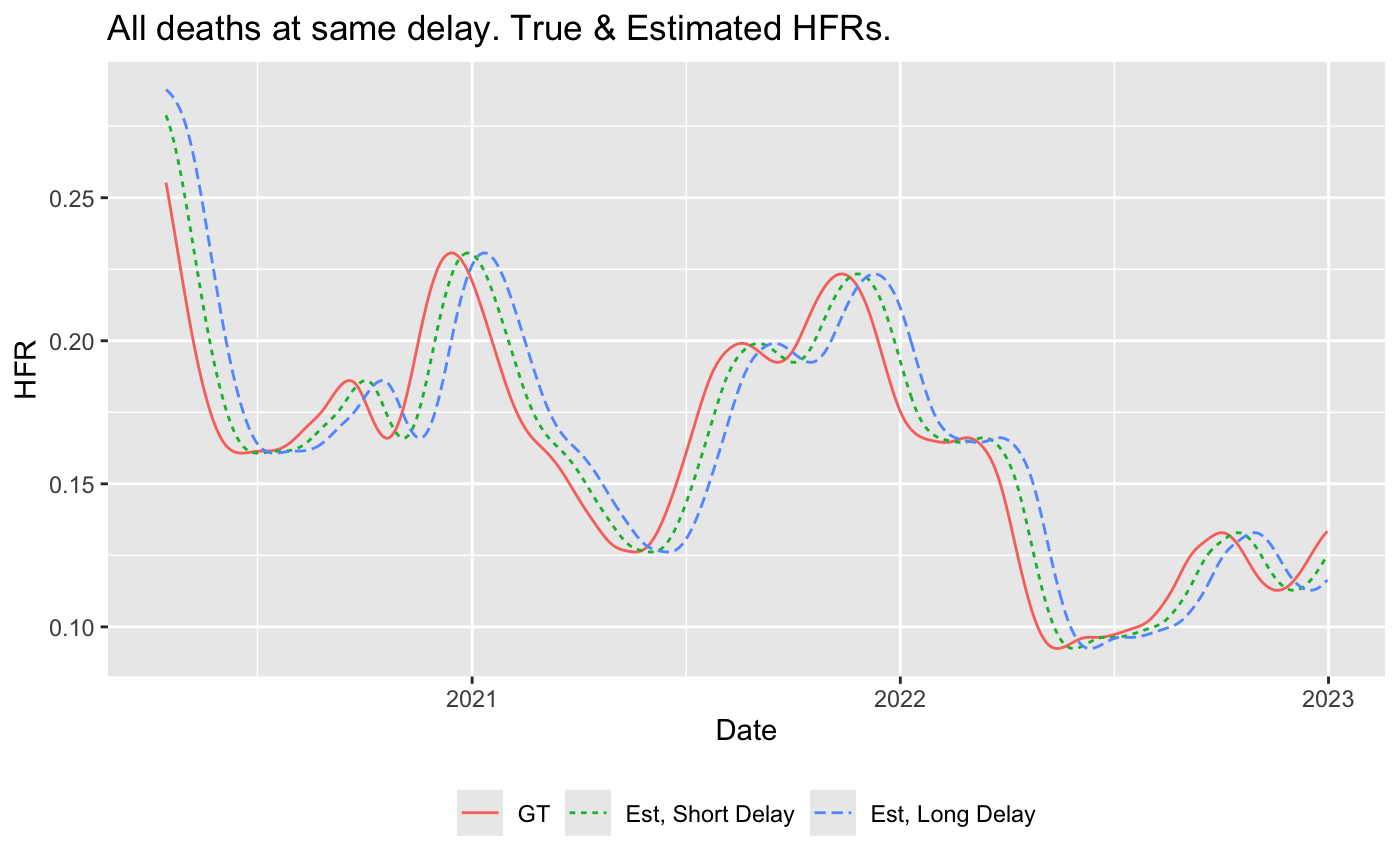
\includegraphics[width=\linewidth]{Figs/sim_onehot.png}
         \caption{All deaths after $\ell$ days. HFR ratios equivalent; plotting delays of $\ell=14$ and 28 days.}
         \label{fig:onehot}
     \end{subfigure}
     \hfill
     \begin{subfigure}[b]{0.45\linewidth}
         \centering
         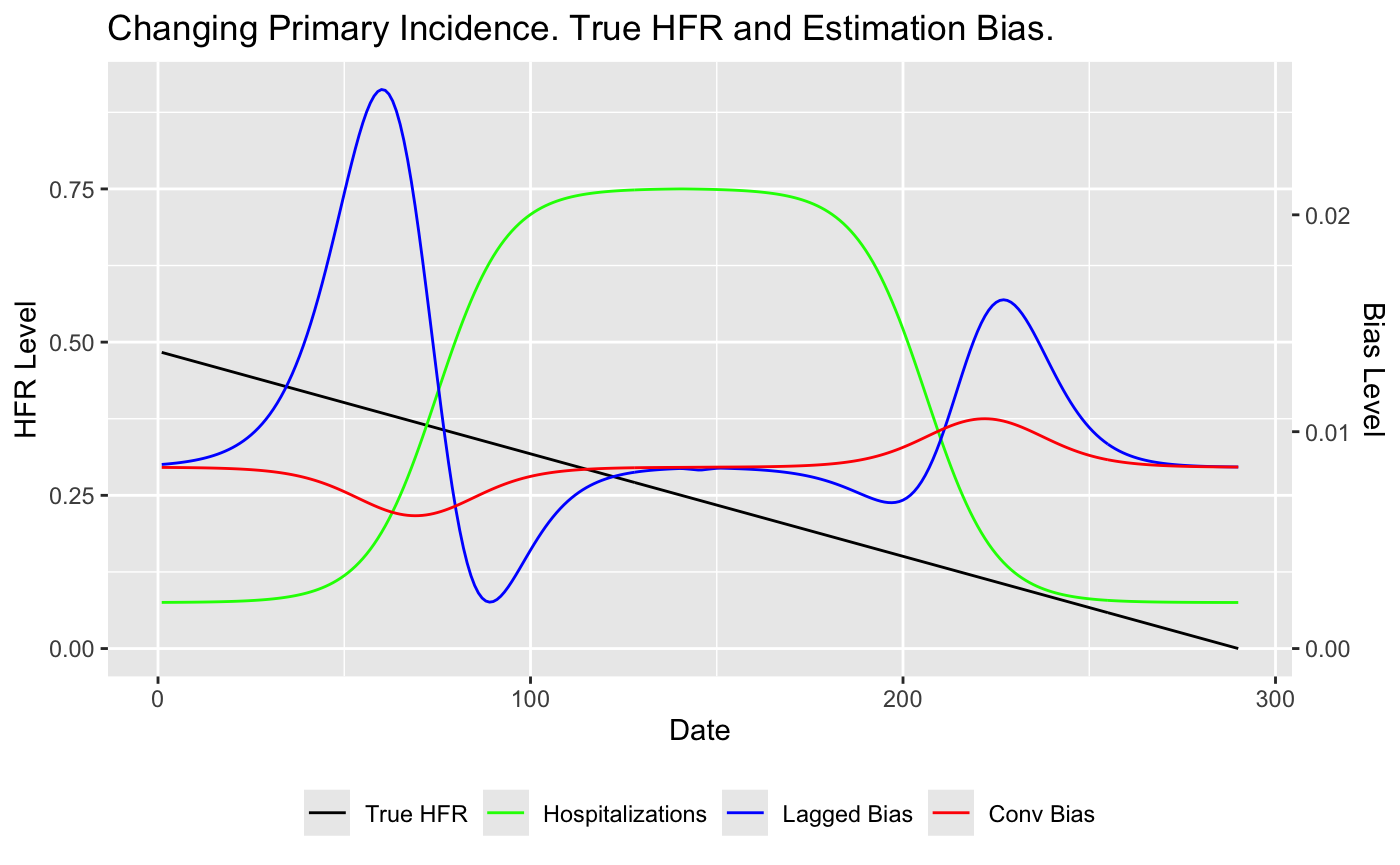
\includegraphics[width=\linewidth]{Figs/sim_chging_primary.png}
         \caption{Changing primary incidence. Plotting bias of lagged and convolutional ratios.}
         \label{fig:chging_primary}
     \end{subfigure}
        \caption{Simple examples of severity rate bias. Analysis in Appendix \ref{apx:analysis}.}
        \label{fig:bias_ex}
\end{figure}


% Empirically, we observe roughly the same biases in the lagged ratio. Its bias expression is highly similar:
This bias expression for the lagged ratio obeys roughly the same structure:

\begin{align}\label{eq:LagBias}
    \text{Bias}(\hat{p}_t^\text{Lagged}) &= \frac{E[Y_t]}{X_{t-L}} - p_t \nonumber\\ 
    &= \frac{\sum_{k=0}^d X_{t-k}\pi_k p_{t-k}}{X_{t-L}} - \frac{X_{t-L} p_t}{X_{t-L}} \nonumber\\
    &= \frac{\sum_{k=0}^d \pi_k\Big( X_{t-k} p_{t-k}-X_{t-L} p_t\Big)}{X_{t-L}}.
\end{align}

\noindent Again, the bias will be positive when the HFR is falling, and vice versa. Indeed, empirically the two ratio estimators are shown to have similar bias (Section \ref{sec:results}). However, Eq. \ref{eq:LagBias} is more difficult to analyze due to its reliance on the lag $L$, hence this section's focus on the convolutional ratio.

\ahcomment{
Can we frame discussion of the bias for the lagged
estimator through Bias Factor 2, 
``shape of the delay distribution'', and use
the fact that the lagged estimator is a
convolution estimator with
$\pi=1\{k=L\}$?  How does that interact with the
Example given for Bias Factor 2?

In fact, in the spirit of Ryan's question, 
``if I were a referee, I would ask how the bias
is affected by different choices of convolutional
kernel in the estimator (if not the oracle),
and by different choices of lag --- would it 
make sense to do \eqref{eq:ConvBias} without 
assuming the oracle delay distribution is known;
obtaining a bias expression that has
separate $\hat\pi$ from oracle $\pi$, and then
specializing it to the cases where we know
the oracle, so $\hat\pi=\pi$, and where
$\hat\pi$ puts all mass on $L$?

I'm not specifically saying this should be done;
just that we should consider doing it if it
streamlines the exposition/clarifies the differences.
}

\rjtcomment{I realized the following: in (5), we're assuming that the convolutional model is well-specified (and that the estimator uses the oracle delay distribution) but in (6), we have not assumed that the lagged model is well-specified. In other words, we've looked at the well-specified bias of the convolutional estimator in (5), but the mis-specified bias of the lagged estimator in (6). I think this is why it's hard to interpret the latter, and creates some confusion.

If we assume that the lagged model is well-specified, the (5) becomes easy to interpret (just like AH says in his comment above ... because in this case can just interpret this in the context of the point \#2 in the discussion of the convolutional estimator). This is a particular (point mass) delay distribution. If this aligns with a big change in the severity rate, then the bias will be high. Right?}

% How do estimates of $\hat\pi$ affect the bias
% and how do different choices of L affect the bias?
% Can it be made arbitrarily large based on certain
% design settings?

\subsection{Experimental Setup}
\subsubsection{HFR Estimation}
% Our experiments focus on the Hospitalization-Fatality Rate (HFR) during COVID-19. While this is a less commonly used metric than the Case-Fatality Rate (CFR), the two should exhibit the same statistical biases. Moreover, CFR may slightly misrepresent our analyses because the model relating cases to deaths may be slightly different. Case reporting during Covid suffered significant time delays, with some cases being reported \textit{after} the death. Therefore, the delay distribution for CFR may not have non-negative support. Unlike case data, the Department of Health and Human Services (HHS) reported hospitalizations in real time based on the date they occurred. This makes hospitalizations a more suitable choice of primary event for study. 

Our experiments focus on the Hospitalization-Fatality Rate (HFR) during COVID-19. Hospitalization reporting was much more complete than case reporting throughout the pandemic. Hospitals were mandated to report new daily admissions to the Department of Health and Human Services (HHS) or face penalties \cite{HHS2023}. The time-to-death delay distribution is indeed supported on integers starting at $k=0$, since hospitalizations are aligned by admission date.

% During the pandemic, data sources counted deaths in different ways. John Hopkins University (JHU) provided the definitive resource for real-time death counts, releasing figures daily. However, these counts reflected the times at which deaths were reported to health authorities, not necessarily when they actually happened. In contrast, the National Center for Health Statistics (NCHS) provide weekly totals for deaths aligned by occurrence. Unlike JHU, the NCHS deaths were not available in real time.

To estimate real-time HFRs, we pulled daily hospitalizations and deaths from the \texttt{epidatr} API, developed by the Delphi Group. Like HHS for hospitalizations \cite{HHS2023}, John Hopkins University (JHU) provided the definitive resource for real-time death counts \cite{JHUepidatr}. These counts reflect the times at which deaths were reported to health authorities, not necessarily when they actually happened. Therefore raw JHU death counts are highly volatile due to reporting idiosyncrasies like day-of-week effects and data dumps. As a result, we used a 7-day trailing average of counts. 

The daily aggregates from each resource were updated over the course of the pandemic. \textbf{TO DO: explain our versioning schema once it's implemented.}

% To estimate real-time HFRs, we use hospitalizations from HHS and deaths from JHU \cite{JHUepidatr}. Data was pulled from the \texttt{epidatr} API, developed by the Delphi Group. Raw JHU death counts exhibit high volatility due to reporting idiosyncrasies like day-of-week effects and data dumps. For that reason, we used a 7-day trailing average of counts. For each dataset, we used the finalized counts, not the versions that would have been available in real time. Doing so would have likely resulted in even more volatile HFR estimates. %We also obtained finalized weekly deaths from NCHS, again smoothing with a spline.

The two ratio estimators (Eq. \ref{eq:lagged} and \ref{eq:conv}) require choices of lag and delay distribution. Appendix \ref{apx:robustness} evaluates the robustness of findings against different hyperparameter values. The experiments in Section \ref{sec:results_real} use a lag of 20 days, which maximizes the cross-correlation between hospitalizations and deaths over all time. We let the delay distribution be a discrete gamma, a common choice. We set its mean to this oracle lag, as lags are often chosen to be the mean of the delay distribution. This mean of 20 matches nicely with a UK study (CITE) that finds a median hospitalization-to-death time of 11 days, and a CDC report that 63\% of COVID deaths are reported within 10 days. We set the standard deviation to 18, because the delay distributions fit by the UK study had standard deviations that were roughly 90\% of their means. 


% However, we set the default choice of lag as 19 days. This is motivated by a UK study finding a median hospitalization-to-death time of 11 days, and a CDC report that 63\% of deaths are reported within 10 days. The convolutional ratio uses an estimate of the hospitalization-to-death delay distribution. A common choice is a discrete gamma distribution, whose standard deviation is comparable to its mean. Empirically, we found a mean of 28 days and standard deviation of 21 days minimized the bias.

\subsubsection{Validation Data}
While the true HFRs are unknown, there are sound ways to approximate them. One such approach is to use line-list HFRs from the National Hospital Care Survey \cite{NHCS2023}. The NHCS recorded weekly HFRs from inpatient deaths in a representative subset of 601 hospitals across the US. %We smoothed these HFRs with a spline to account for inter-week variability. 
% \ahcomment{
%     % Do you mean ``intra-week variability'' here?  inter-week variability
%     % is what we want to have remain right?
%     % Yes, thanks for the catch!
%     Also --- genuinely curious --- why did we use a spline 
%     rather than just a 7-day moving average?
%     \textcolor{blue}{The NHCS HFRs were reported weekly, and had a fairly high degree of noise.}
% }

HFRs from aggregate hospitalization and death counts are significantly higher than those from NHCS because not all deaths occur in hospitals. A CDC analysis reported the percentage of inpatient deaths every month from 2020 through 2022; roughly 60\% of Covid deaths occurred in hospitals in 2022, down from nearly 70\% in 2021 and 2022. To account for non-inpatient deaths, we divided the NHCS curve by these percentages. Finally, we smoothed the resulting HFRs with a spline. To do so, we used the \texttt{smooth.spline} function in \texttt{R}, which chooses the smoothness hyperparameter with generalized cross validation. % after again smoothing with a spline. 
% NOTE: The more principled thing to do is to divide by proportion of in-patient deaths L days from each timestep, because hospitalizations at t effect deaths after t. But this is more work to explain.

% Let $\eta_t$ be the unscaled, smoothed NHCS HFRs. I'm not sure whether this is forward- or backward-looking; it just says it's the percentage of confirmed COVID-19 hospital encounters with a discharge status of in-hospital death, presented each week. I think this is forward looking? So they look at all hospitalizations for a given week with known discharge status, and calculate the rate that are deaths?

% Number of deaths should be roughly number of hospitalizations * average HFR. So had scaled $\bar Y = \bar X * c \bar\eta \Leftrightarrow c = \frac{\bar Y}{\bar{\eta} \bar X}$. This didn't quite work, though, since the proportion of in-hospital deaths changes over time. That it falls in 2022 indicates there should be a higher scaling rate to the HFRs, for example. 

% Assuming the NHCS HFRs are forward-looking and the lagged model is correct (lol), the number of inpatient deaths $Y_{t+L}^{in}\approx X_t \eta_t$. Let $s_t$ be the proportion of deaths that die in-hospital at $t$ (this is reported in a monthly window surrounding $t$). Then $s_t Y_t \approx Y_t^{in}$. So $Y_{t+L} \approx \frac{X_t \eta_t}{s_{t+L}}$. That is, I can use $\eta_t/s_{t+L}$ as the HFRs, and ultimately rescale as before if needed. 

We considered two other sources for ground truth HFRs, discussed in Appendix \ref{apx:alt_gt}. Unlike NHCS, these HFRs are obtained from aggregate counts, not line-list data. Fortunately, they are fairly consistent with the rescaled NHCS data, bolstering our trust in it. Of course, the NHCS curve is merely an approximation for the ground truth; its values, especially after mid-2022, may be incorrect. Nevertheless, it is a useful aide with which to judge the fidelity of our HFR estimates.
% but entail making worse assumptions. 

\section{Results}\label{sec:results}

\subsection{National COVID Data}\label{sec:results_real}

% \begin{figure}
%     \centering
%     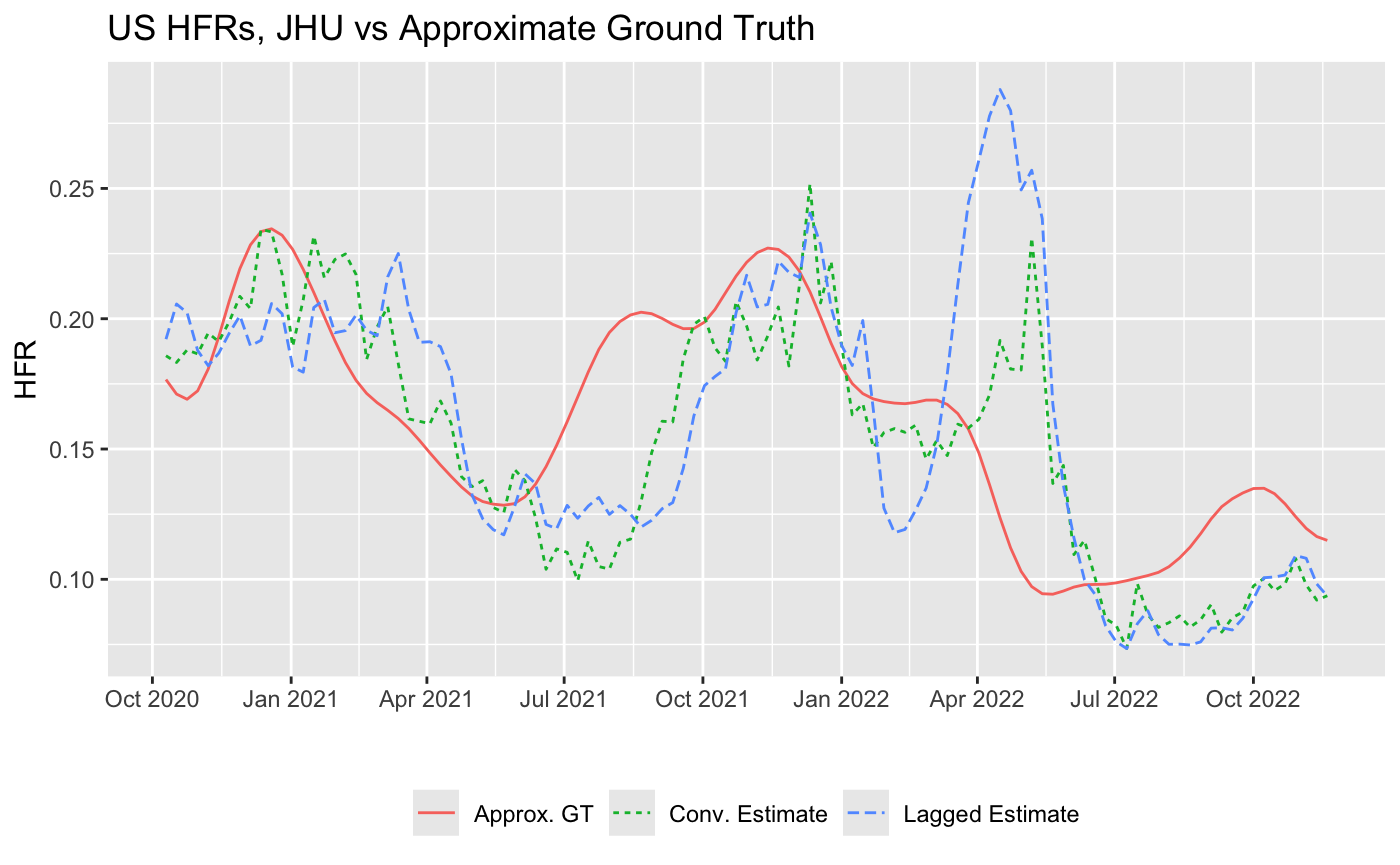
\includegraphics[width=0.8\linewidth]{Figs/US_ests_vs_GT.png}
%     \caption{Time-varying HFR estimates are highly biased. Terms in both ratio estimates are smoothed over a 7-day window.}
%     \label{fig:basic_est_vs_gt}
% \end{figure}

\begin{figure}
     \centering
     \begin{subfigure}[b]{0.55\linewidth}
         \centering
         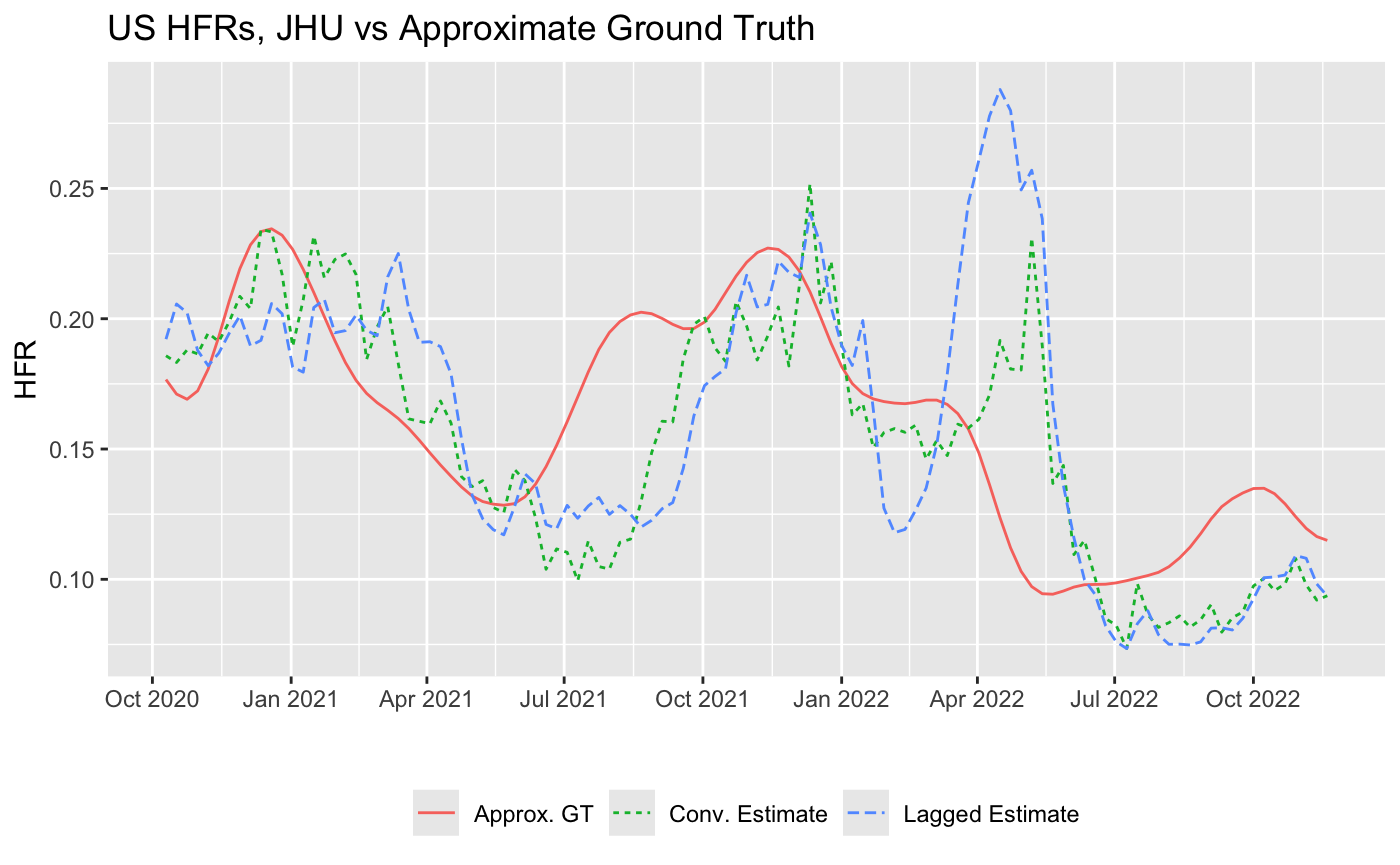
\includegraphics[width=\linewidth]{Figs/US_ests_vs_GT.png}
         \caption{Comparing convolutional and lagged ratios against approximate ground truth, Oct. 2020 - Dec 2022.}
         \label{fig:basic_est_vs_gt}
     \end{subfigure}
     \hfill
     \begin{subfigure}[b]{0.4\linewidth}
         \centering
         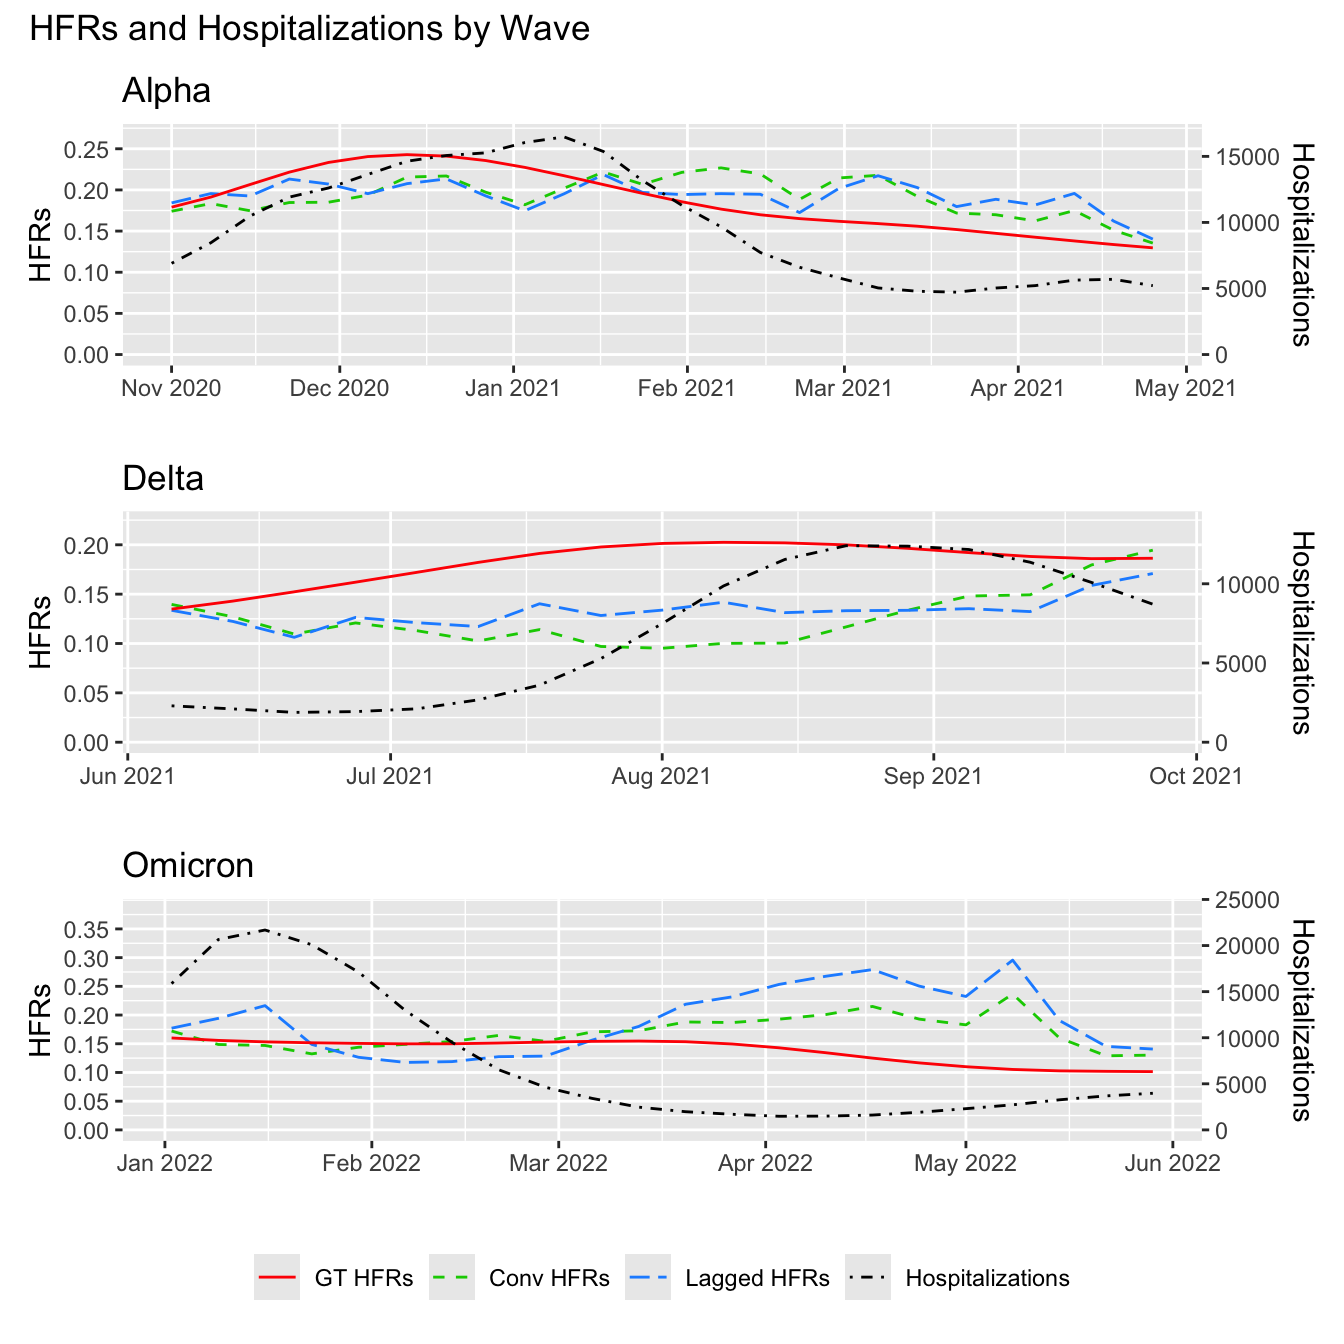
\includegraphics[width=\linewidth]{Figs/hfrs_by_wave.png}
         \caption{HFRs and hospitalizations in three periods with major bias.}
         \label{fig:wave}
     \end{subfigure}
        \caption{Convolutional ratio estimates are biased regardless of which delay distribution is selected.}
        \label{fig:basic_est_vs_gt_figs}
\end{figure}

Figure \ref{fig:basic_est_vs_gt_figs} highlights the bias of these ratio estimators. Both the lagged and convolutional ratios respond very slowly to changes in the HFR. As the HFR declines throughout the Alpha wave in early 2021, both ratios stay around 0.2 for several months. More troublingly, they are very slow to detect the rising HFR in the early Delta period (summer 2021). %A central purpose of these estimators is to inform stakeholders of increased risks in real time; this indicates a failure to do so during the Delta surge.

The most significant bias comes in the middle of the Omicron wave in spring 2022. The true HFRs sharply decline in this period, from a high of roughly 17\% in March to a low of 9\% only two months later. At the same time, the HFR estimates \textit{rise}, peaking over 20\% as the true HFR reaches its nadir. This dramatic surge signals a serious false alarm. 

The analysis in Section \ref{sec:analysis} explains for these three failure cases. Recall the bias moves in the opposite direction of the true severity rate. Rising HFRs engender negative bias, hence the delayed rise in the Delta wave. Falling HFRs correspond to positive bias, as observed in early 2021 and 2022. In addition, the enormity of the bias during Omicron can be attributed to the precipitous decline in hospitalizations, as falling primary incidence has been shown to exacerbate the bias. Average daily hospitalizations declined from over 20,000 in mid-January to only 1,500 by April 1. Finally, the delay distribution is relatively long with JHU deaths due to its alignment by report date. This is shown to have a substantial impact on the bias, as analyzed in Appendix \ref{apx:NCHS_deaths}
\ahcomment{
This is great --- I think we would really drive the point home
if in addition to Figure 1, we had a three-panel figure that
``zooms in'' on each of these cases, and specifically labels them
with each of the three failure modalities, so that the reader
can see exactly how they correspond to the conditions under
which bias occurs outlined in Section 2. \textcolor{blue}{How's this look?}%  (Even better if there are toy examples in Section 2, so the reader can see the ``idealized version'' of the failure, and a ``real world'' manifestation of that failure mode.
}

We performed several robustness checks to assess the stability of these findings. Figure \ref{fig:basic_est_vs_gt} compares the convolutional and lagged ratio estimators, finding bias in both. The convolutional estimator is slightly better, but still very problematic. Appendix \ref{apx:robustness} explores the effect of different hyperparameters and locations. By and large, the ratio estimators are biased regardless of these considerations. 

\subsection{Simulated Data}


We further evaluated these methods on simulated deaths whose true HFRs is known. Throughout these experiments, we used observed, finalized HHS hospitalization reports $X_t$, and various models for the HFR and delay distribution. Given a series of time-varying HFRs $p_t$ and delay distribution $\pi$, deaths are defined without noise as according to \ref{eq:model}

$$Y_t := \sum_{k=0}^d X_{t-k} \mathbb{P}(\text{die at $t$ }\vert\text{ hosp at }t-k) = \sum_{k=0}^d X_{t-k} \pi_k p_{t-k}.$$

To mimic the real data, we first used the same HFRs from NHCS used for validation in \ref{sec:results_real}. We also inverted them and rescaled in order to simulate the opposite trend. Lastly, we explored a stationary HFR of 10\% over all time. The delay distributions were again gamma with standard devation 0.9 of their mean. We experimented with means of 12 and 24 to illustrate a short and long delay distribution. The ratio estimators used the oracle hyparameters: The true delay distribution for the convolutional ratio, and its mean for the lagged method. Estimates were not smoothed over a trailing window.
% In addition, we used the delay distributions that produced the most reasonable convolutional HFRs on the observed death counts. For NCHS, this was a gamma distribution with mean 11 and standard deviation 10; for JHU, these quantities were 28 and 21, respectively.  (TO DO: replace all this.)

\begin{figure}
    \centering
    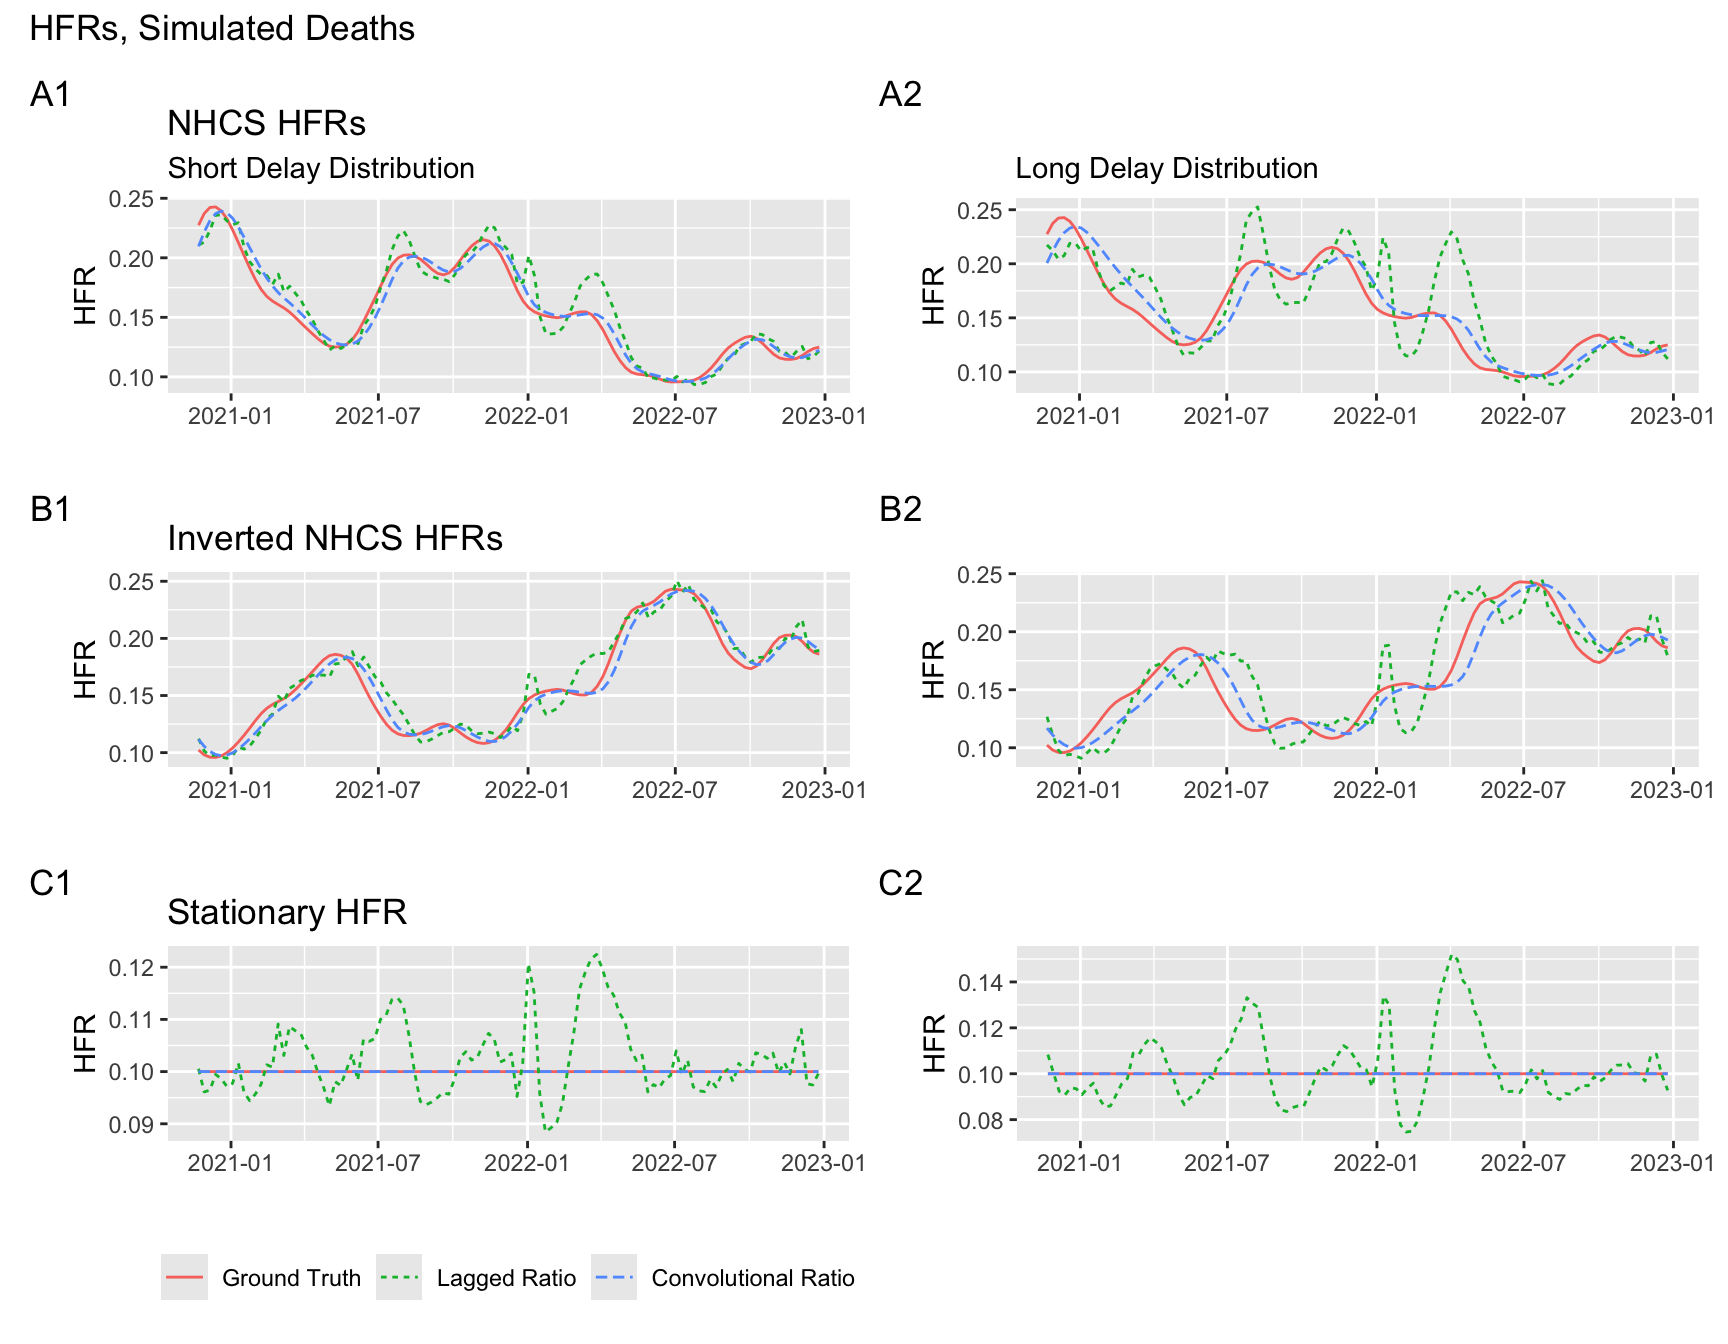
\includegraphics[width=0.9\linewidth]{Figs/simulated_results2.png}
    \caption{True and Estimated HFRs from Simulated Deaths. First column has short delay distribution, second has long.}
    \label{fig:sims}
\end{figure}

Figure \ref{fig:sims} displays the results on the 2 delay distributions and 3 HFR settings. The bias was significantly more pronounced with the longer delay distribution. To assess the relationship between the estimated and true HFRs, we identified the offset that maximized the cross-correlation between the two series. On both the true and inverted NHCS HFRs, this was 7 days for the short distribution, a relatively innocuous gap. However, the offset is 21 days with the longer distribution - concerningly slow during a rapidly changing severity rate like the Delta surge.

Interestingly, the lagged estimator performed considerably worse than the convolutional ratio. When the true HFR changed, the lagged estimates oscillated while the convolutional ratio followed the general trend. In the stationary HFR case, its bias reached as high as 50\%; in contrast, the convolutional estimator was unbiased as anticipated (Eq. \ref{eq:ConvBias}). This discrepancy is striking, as the lagged ratio is the most commonly-used time-varying estimator. 

\section{Discussion}

Our analyses illustrate that practitioners should take caution when using these time-varying severity ratios. They exhibit considerable bias when severity rates change, particularly the popular lagged ratio. A major purpose of these estimators is to inform stakeholders of changing risks in real time; this bias indicates they may fail to do so in a reliable manner.

Given the drawbacks of these methods, alternative approaches may be preferable when there is reason to believe the true rate is changing. If possible, severity rates can be obtained from line-list data after accounting for right censoring. These rates can then be scaled to a broader population with careful demographic adjustment \cite{verity2020estimates}. 

% Other methods exist to estimate severity rates from aggregate data. 
% When only aggregate data is available, 
More commonly, only aggregate data is available, especially in real time. In that case, other methods may outperform these ratios. \citeauthor{fusedlasso} propose estimating all severity rates at once with a Fused Lasso model, using the relation in Eq. \ref{eq:model}. Unlike the other approaches, this method is inherently forward-looking, where rates at $t$ are exclusively used to produce secondary events after $t$. However, it may suffer from other sources of bias. It is inclined to estimate smoothly-changing severity rates as piecewise constant, and may yield unstable real-time estimates due to scarce data at the tail.

\citeauthor{UKpaper} also proposed a forward-looking method, this one a ratio between relevant primary and secondary events. However, this method is not applicable in real time, as it uses secondary events after $t$ to compute the severity rate. Nevertheless, it is a useful tool for retrospective estimation. 

% TO DO: FIX
Another retrospective tool is aggregate COVID deaths from NCHS, a resource that was not available in real time (Appendix \ref{apx:NCHS_deaths}). Unlike JHU, whose aggregates align deaths by report date, NCHS counts deaths on the day the actually occurred. As a result, the mean of its delay distribution is considerably lower, so it produces more accurate ratio estimates (Fig. \ref{fig:jhu_vs_nchs}, \ref{fig:sims}). Analogously, bias is a more serious issue with earlier primary events. For example, case- or infection-fatality ratios may be more biased than hospitalization-fatality ratios. 

% In a similar vein, deaths from NCHS should be used for retrospective analysis, not JHU. Longer delay distributions have been shown to produce significantly more bias (Fig. \ref{fig:jhu_vs_nchs}, \ref{fig:sims}). Therefore estimates with data that counts secondary events by report date will always be worse. Analogously, bias is a more serious issue with earlier primary events. For example, case- or infection-fatality ratios may be more biased than hospitalization-fatality ratios. 

While still biased, the convolutional ratio generally outperformed the lagged method (Fig. \ref{fig:basic_est_vs_gt}, \ref{fig:sims}). While this estimator is widely used for overall HFRs with cumulative counts, we have not come across any applications for the time-varying case. This further suggests the lagged ratio is overused in practice, though the convolutional ratio may not be the best existing alternative \cite{fusedlasso, UKpaper}.

TO DO: Discuss other sources of bias in severity rates. e.g. Anastasios, Nick Reich papers.

An interesting connection exists between estimating severity rates and reproduction numbers. A central metric in epidemiology is \textit{case} $R_t$, the average number of secondary infections produced by a single infection at time $t$. Typically estimated in real-time is the closely-related \textit{instantaneous} $R_t$, average number of secondary infections at time $t$ produced by a single primary infection in the past. Comparable to the delay distribution $\pi$ is the renewal equation $g$, which measures the time between primary and secondary infections.

As defined in \ref{eq:severity}, the severity rate is analogous to case $R_t$. Both concern the average number of secondary events produced by a primary event at time $t$. Moreover, the real-time severity ratios we study are analogous to instantaneous $R_t$, both of which measure how primary events in the past contribute to secondary events at $t$. Indeed, one of the most popular frameworks for estimating instantaneous $R_t$ is strikingly similar to the convolutional ratio \cite{fraser2007,wallinga2007how,cori2013new}:
\begin{equation}\label{eq:instRt}
    \hat{R_t} = \frac{I_t}{\sum_{k=0}^d I_{t-k}g_k}.
\end{equation}
% The most fundamental difference between Eq. \ref{eq:instRt} and \ref{eq:conv} is the former expresses the rate for a single time series. 
\citeauthor{fraser2007} notes that instantaneous $R_t$ is equal to case $R_t$ if conditions remain unchanged. Similarly, we demonstrated that the convolutional ratio \ref{eq:conv} is unbiased if the severity rate and delay distribution in the $d$ days before $t$ are stationary. Bias arises as a consequence of changing conditions. Future work could apply this same analytical framework to $R_t$, examining the fidelity of instantaneous $R_t$ as a proxy for case $R_t$. 


\bibliographystyle{apalike}
\bibliography{refs}

\pagebreak
\appendix
\section{Simulation Analysis}\label{apx:analysis}

To elucidate the extent to which changing severity rates bias the convolutional ratio, consider the trivial case where all secondary events occur after exactly $\ell$ days with no noise. By definition, $\pi_k = \mathds{1}\{k=\ell\}$, so the convolutional and lagged ratios are both $\hat{p}_t = \frac{X_{t-\ell}p_{t-\ell}}{X_{t-\ell}} = p_{t-\ell}$. In this case, the bias is the change in the true severity rate $p_{t-\ell} - p_t$. The estimator is unbiased only when the severity rate is stationary. Otherwise, for example, the ratio will be 20\% too low if the true severity rate was 20\% lower $\ell$ days ago. Figure \ref{fig:bias_ex} displays this with the approximate ground truth HFRs from NHCS. 

Intuitively, severity rates are liable to be less similar to the present value $p_t$ further back in time. Therefore heavier-tailed delay distributions should have more bias. In the above example, the bias $p_{t-\ell}-p_t$ is generally larger when $\ell=28$ than $\ell=14$ (Fig \ref{fig:onehot}). Constructing another simple case, consider a severity rate that changes monotonically before $t-m$, then is constant until $t$. If the delay distribution assigns all probability mass within the first $m$ days, the convolutional ratio will be unbiased at $t$. Otherwise, it will be biased, with longer delay distributions producing greater bias. 

Section \ref{sec:analysis} claims that changes in primary incidence levels affect the magnitude of bias for the convolutional ratio. Here, we present a simple example that formalizes this claim. Suppose half of the secondary events occur immediately after the primary event ($t=0$), and the other half after $\ell$ days. Further assume $p_{t-\ell}\neq p_t$, so there is some degree of bias. Then
\begin{align*}
    \lvert\text{Bias}(\hat{p}_t^{\text{Conv}})\rvert &= \frac{\frac{1}{2}\big\lvert X_{t}(p_t-p_t) + X_{t-\ell}(p_{t-\ell}-p_t)\big\rvert}{\frac{1}{2}(X_{t}+X_{t-\ell})} \\
    &=\frac{X_{t-\ell}\lvert p_{t-\ell}-p_t\rvert}{X_{t-\ell}(1+\frac{X_{t}}{X_{t-\ell}})} = \frac{\lvert p_{t-\ell}-p_t \rvert}{1+\frac{X_{t}}{X_{t-\ell}}}
\end{align*}

The absolute bias is monotonically decreasing in $\frac{X_{t}}{X_{t-\ell}}$, the proportion change in primary incidence. Rising primary incidence ($\frac{X_{t}}{X_{t-\ell}}>1)$ yields less bias, while falling levels yield more.

Figure \ref{fig:chging_primary} displays this setting. Hospitalizations are defined as $X = \sigma(s)*9000+1000$, where $\sigma$ is the sigmoid function and $s$ takes 300 evenly spaced steps from -9 to 7. The true HFRs fall from 0.5 to 0 over the same number of even steps. Indeed, the convolutional ratio's bias dips as hospitalizations rise, and rises as they fall. 

When daily hospitalizations approach a constant level, the two estimators become the same ratio, so their biases converge. During periods of change, however, the lagged estimator has different bias. It oscillates up and down, reaching higher bias than the convolutional ratio. 

TO DO: ANALYZE WHY THIS HAPPENS.

\section{Retrospective Deaths}\label{apx:NCHS_deaths}

JHU presented daily deaths in real time, aligned by the date they were reported. In contrast, the National Center for Health Statistics (NCHS) provided weekly totals for deaths aligned by occurrence, and were not available in real time. Thus, delay distributions with NCHS deaths have a lighter tail. 

Figure \ref{fig:jhu_vs_nchs} shows this minor change has a significant effect on the bias. It compares the real-time lagged ratios (Eq. \ref{eq:lagged}) with deaths sourced from JHU and NCHS. JHU is much more biased during the Alpha, Delta, and Omicron periods discussed. For example, NCHS only rises from 12\% to 14\% as Omicron falls, far below JHU's surge above 25\%. As analyzed in \ref{sec:analysis}, JHU's heavier-tailed delay distribution inflates the influence of dates with higher HFRs than the present.

% The shape of the delay distribution plays a significant role in the bias. 

\begin{figure}
    \centering
    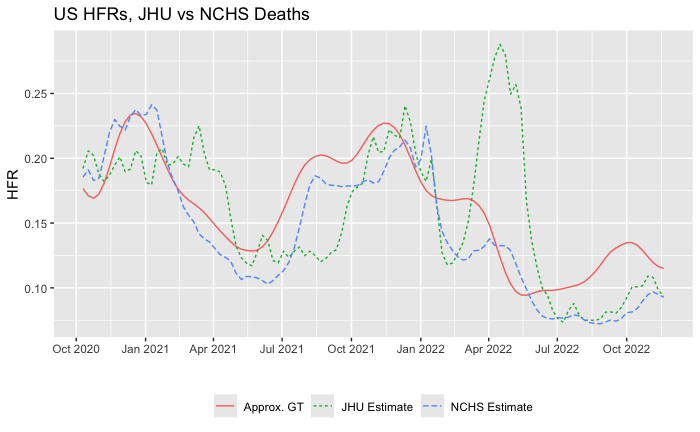
\includegraphics[width=0.7\linewidth]{Figs/jhu_vs_nchs.png}
    \caption{Real-time Lagged Ratios, JHU vs NCHS deaths. Seven-day smoothing with 19- and 11-day lags, respectively.}
    \label{fig:jhu_vs_nchs}
\end{figure}


\section{Alternative Ground Truth}\label{apx:alt_gt}

\begin{figure}
    \centering
    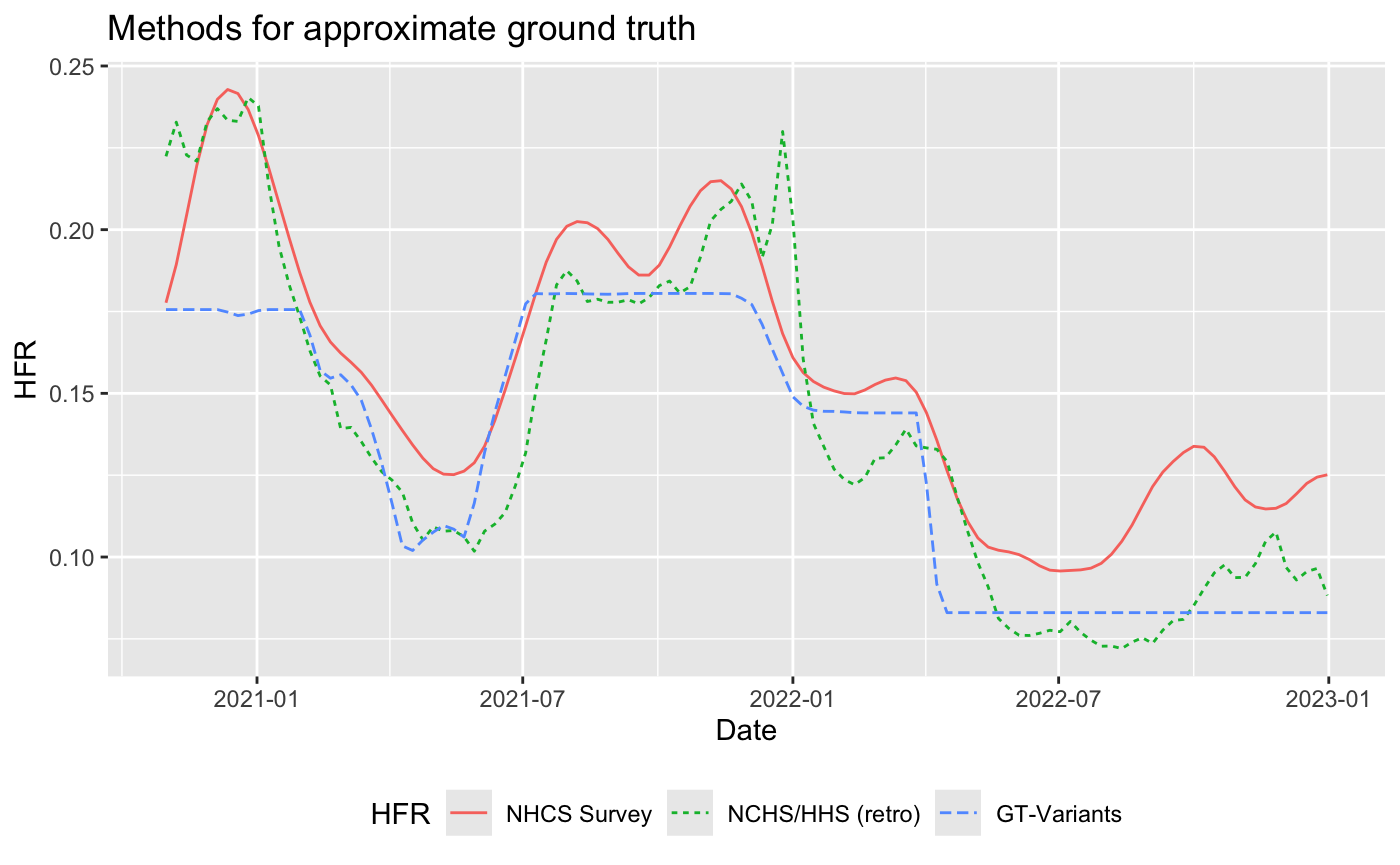
\includegraphics[width=0.8\linewidth]{Figs/ApproxGT.png}
    \caption{Methods for Retrospective Ground Truth HFRs.}
    \label{fig:approxGT}
\end{figure}

We considered two retrospective approaches to approximate the ground truth national HFRs over time. The first approach took lagged ratios with aggregate deaths from NCHS. NCHS is a better resource than JHU because it uses death counts from the date they actually occurred, not merely reported. In addition, we take a forward-looking ratio, which is retrospective insofar as it uses data after time $t$ to estimate the HFR.
% Unlike the real-time estimates, we  method is forward-looking and . 

\begin{equation}\label{eq:LaggedRetro}
    \hat{p}_t^{\text{LaggedRetro}} = \frac{Y_{t+L}}{X_t}
\end{equation}
% \noindent Equation \ref{eq:LaggedRetro} is retrospective because it uses data after time $t$, and therefore is not applicable in real-time. 

The second approach computed a single HFR for each major variant, then mixing by the proportions of variants in circulation. Formally, let $\hat{p}_j$ approximate the HFR of variant $j$; let $v_t^j$ be its proportion of cases at time $t$, where $\sum_j v_t^j = 1 \; \forall t$. The HFR estimate is

$$\hat{p}_t^{\text{Var}} = \sum_j v_t^j \hat{p}_j.$$

Each variant's HFR $\hat p_j$ was defined as the ratio of total NCHS deaths and HHS hospitalizations during the period where it accounted for over 50\% of activate cases. The case proportions $v_t^j$ were obtained from \texttt{covariants.org}. To ensure estimates were reasonable, we only considered the 4 largest variants: The original strain, Alpha, Delta, and Omicron. Because Omicron began with an enormous surge that quickly subsided, we split it into early and late periods at April 1, 2022, following \cite{adjei2022mortality}.

Figure \ref{fig:approxGT} displays the three curves approximating the true HFRs. They have nontrivial differences in magnitude, but move more or less in conjunction. To validate our results, we primarily used the rescaled NHCS HFRs as the least problematic of the three. The retrospective NCHS ratios are subject to statistical bias, expressed in \ref{eq:LagBias}. The variant-based HFRs are flatter, as they do not account for other sources of variability. Therefore, they do not explain for the statistical bias within each variant period, which arises due to changes in the underlying severity rate.  %unreasonably flat

\section{Robustness Checks}\label{apx:robustness}
\subsection{Hyperparameters}
In this section we demonstrate the robustness of our findings against choices of hyperparameters. (All results are with the finalized version of JHU deaths.) First, Figure \ref{fig:window} plots performance over choices of window size parameter. We analyze smoothed versions of the lagged estimator

\begin{equation}\label{eq:laggedSmooth}
    \hat{p}_t^\text{Lagged,W} = \frac{\sum_{s=t-w+1}^{t} Y_s}{\sum_{s=t-w+1}^{t} X_{s-\ell}},
\end{equation}
\noindent as well as the convolutional estimator
\begin{equation}\label{eq:convSmooth}
    \hat{p}_t^\text{Conv,W} = \frac{\sum_{s=t-w+1}^{t} Y_s}{\sum_{s=t-w+1}^{t} \sum_{k=0}^d X_{s-\ell-k}\hat\pi_k}.
\end{equation}

\noindent Results are very similar, indicating the bias does not disappear when smoothing over a longer history. 

\begin{figure}
    \centering
    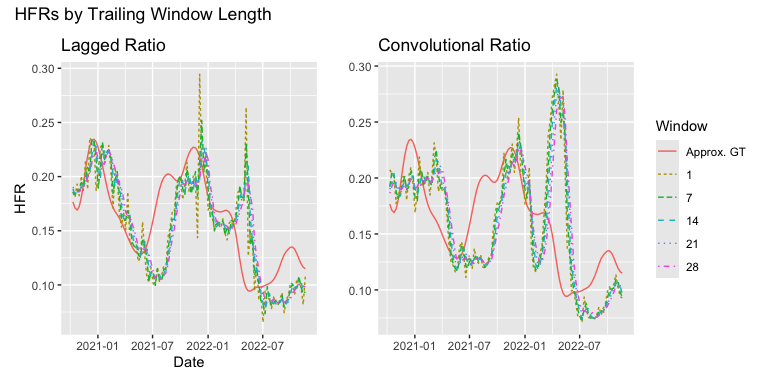
\includegraphics[width=0.75\linewidth]{Figs/window_size.png}
    \caption{The length of the trailing window bears little impact on the findings.}
    \label{fig:window}
\end{figure}

We next examine the time-to-death hyperparameters: The lag $L$ for the lagged ratio and delay distribution $\pi$ for the convolutional ratio. Figure \ref{fig:lag} displays HFR estimates with lags ranging from 2 to 5 weeks. Unlike the window size, changing this parameter leads to different behavior across lags. Some choices are better than others; a 28-day lag, for example, falls appropriately during Alpha and rises less slowly during Alpha. However, all are biased to varying degrees, most notably the huge spurious surge in spring 2022.

\begin{figure}
    \centering
    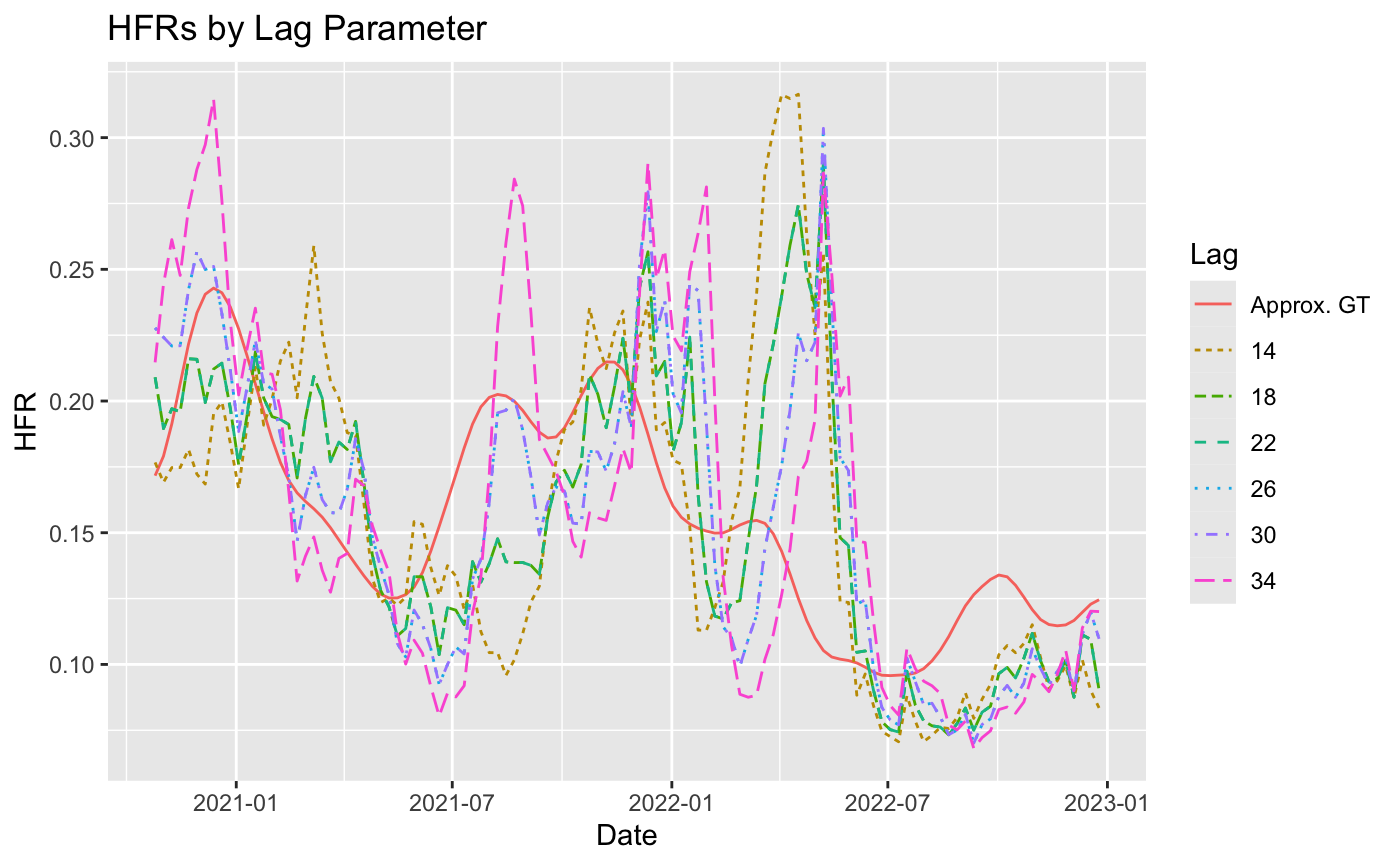
\includegraphics[width=0.7\linewidth]{Figs/hfrs_by_lag.png}
    \caption{HFRs are biased regardless of what lag parameter is selected.}
    \label{fig:lag}
\end{figure}

% TO DO: Different delay distribution
Figure \ref{fig:delays} compares the performance of the convolutional ratio across different choices of delay distribution. We kept the discrete gamma shape for each, but varied the mean and standard deviation. As before, Figure \ref{fig:delay1} kept the standard deviation to 90\% of the mean, per \citeauthor{UKdelay}. We also evaluated with a more compact delay distribution in \ref{fig:delay2}. 

% \begin{figure}
%     \centering
%     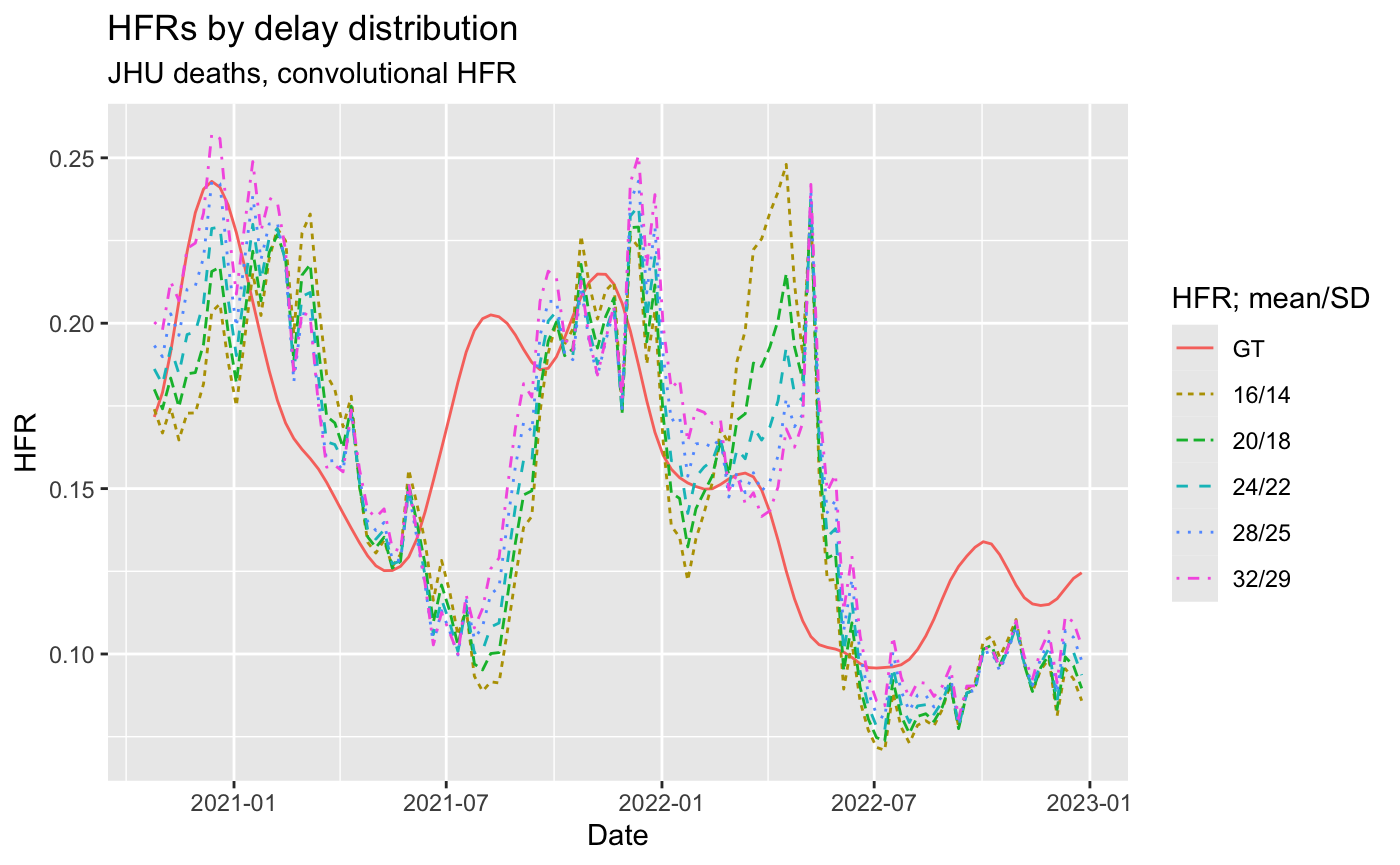
\includegraphics[width=0.7\linewidth]{Figs/hfrs_by_delay.png}
%     \caption{HFRs are biased regardless of what delay distribution is selected.}
%     \label{fig:delay}
% \end{figure}

\begin{figure}
     \centering
     \begin{subfigure}[b]{0.45\linewidth}
         \centering
         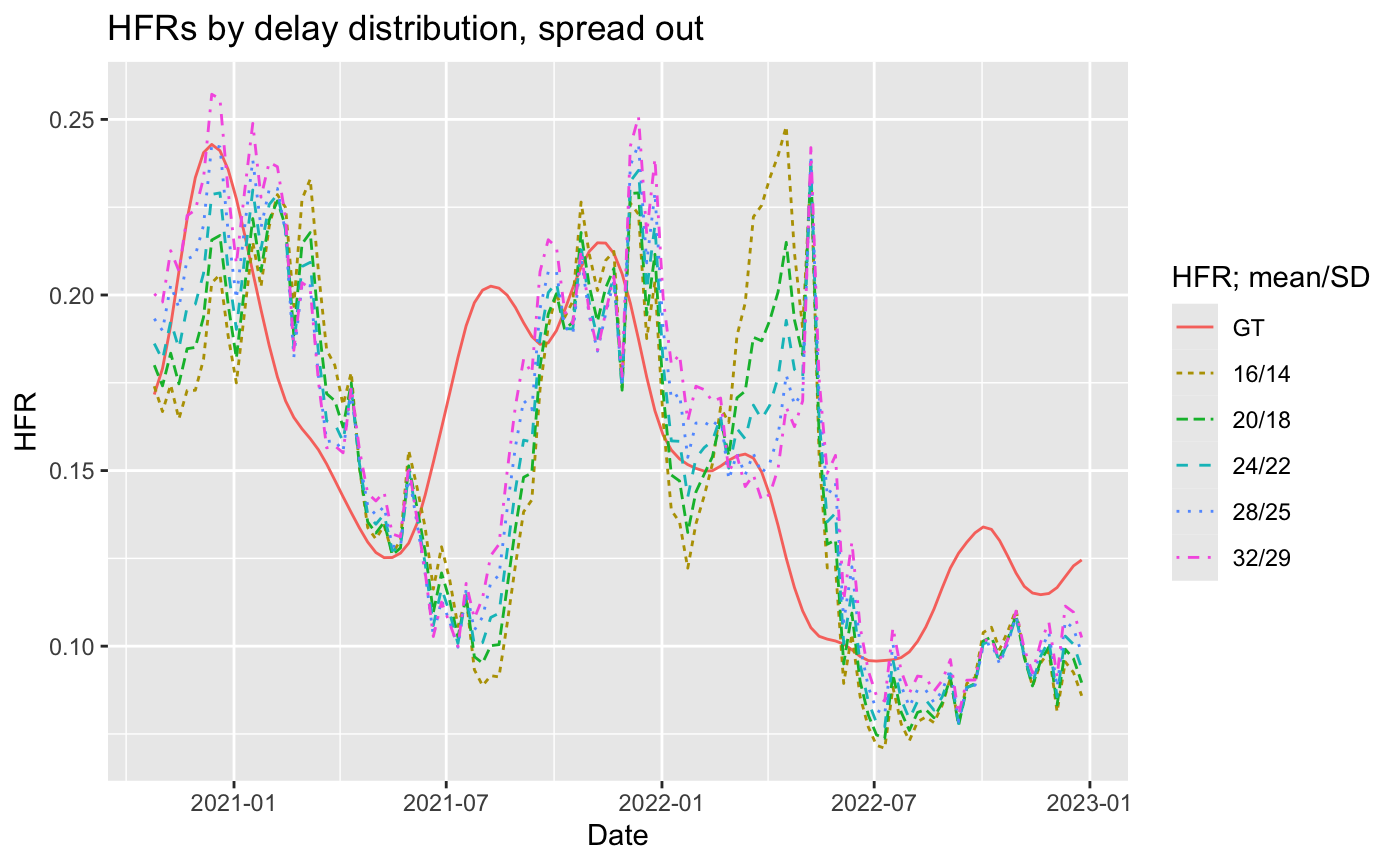
\includegraphics[width=\linewidth]{Figs/hfrs_by_delay1.png}
         \caption{SD is $0.9\times$mean.}
         \label{fig:delay1}
     \end{subfigure}
     \hfill
     \begin{subfigure}[b]{0.45\linewidth}
         \centering
         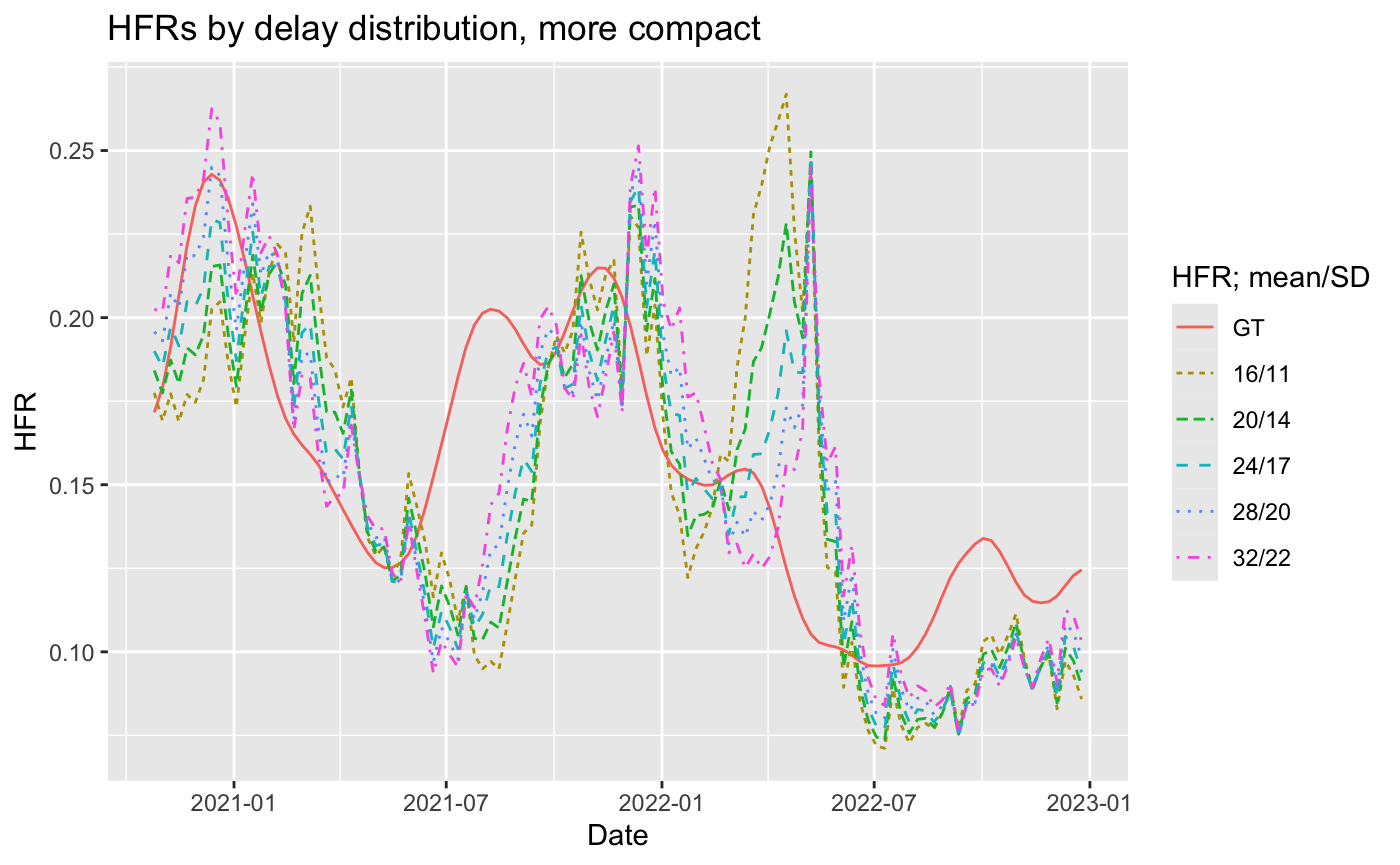
\includegraphics[width=\linewidth]{Figs/hfrs_by_delay2.png}
         \caption{SD is $0.7\times$mean.}
         \label{fig:delay2}
     \end{subfigure}
        \caption{Convolutional ratio estimates are biased regardless of which delay distribution is selected.}
        \label{fig:delays}
\end{figure}
All HFR estimates in the figures are significantly biased. Regardless of delay distribution, the ratios are negatively biased during the onset of Delta, and surge after the peak of Omicron. This indicates the bulk of the error is fundamental to the estimator, and cannot be attributed to model misspecification. 

Comparing to the approximate ground truth HFRs from NHCS, performance improved slightly with a longer delay distribution than the purported mean of 20 days. Its mean absolute error was 0.031, whereas the delay distribution with mean 28 and standard deviation 25 had a MAE of 0.27. Nevertheless, this difference is relatively small, with the alternative delay distribution still showing similar bias.

\subsection{Geography}

Next, we repeat our analysis on different geographies, finding similar trends. We repeated our computations on the 6 largest US states with the same lag and delay distribution, with finalized death counts from JHU. Because the NHCS survey was conducted on a subset of hospitals meant to represent the US at large, it may poorly approximate the HFRs for individual states. A better state-level source is the retrospective lagged estimate (\ref{eq:LaggedRetro}) using NCHS deaths. Figure \ref{fig:state-level} compares this rough ground truth with the real-time estimates. For both NCHS and JHU deaths, we again take the lag that maximizes cross-correlation with hospitalizations; the standard deviation of the delay distribution is 0.9 times the mean. 

 \begin{figure}
     \centering
     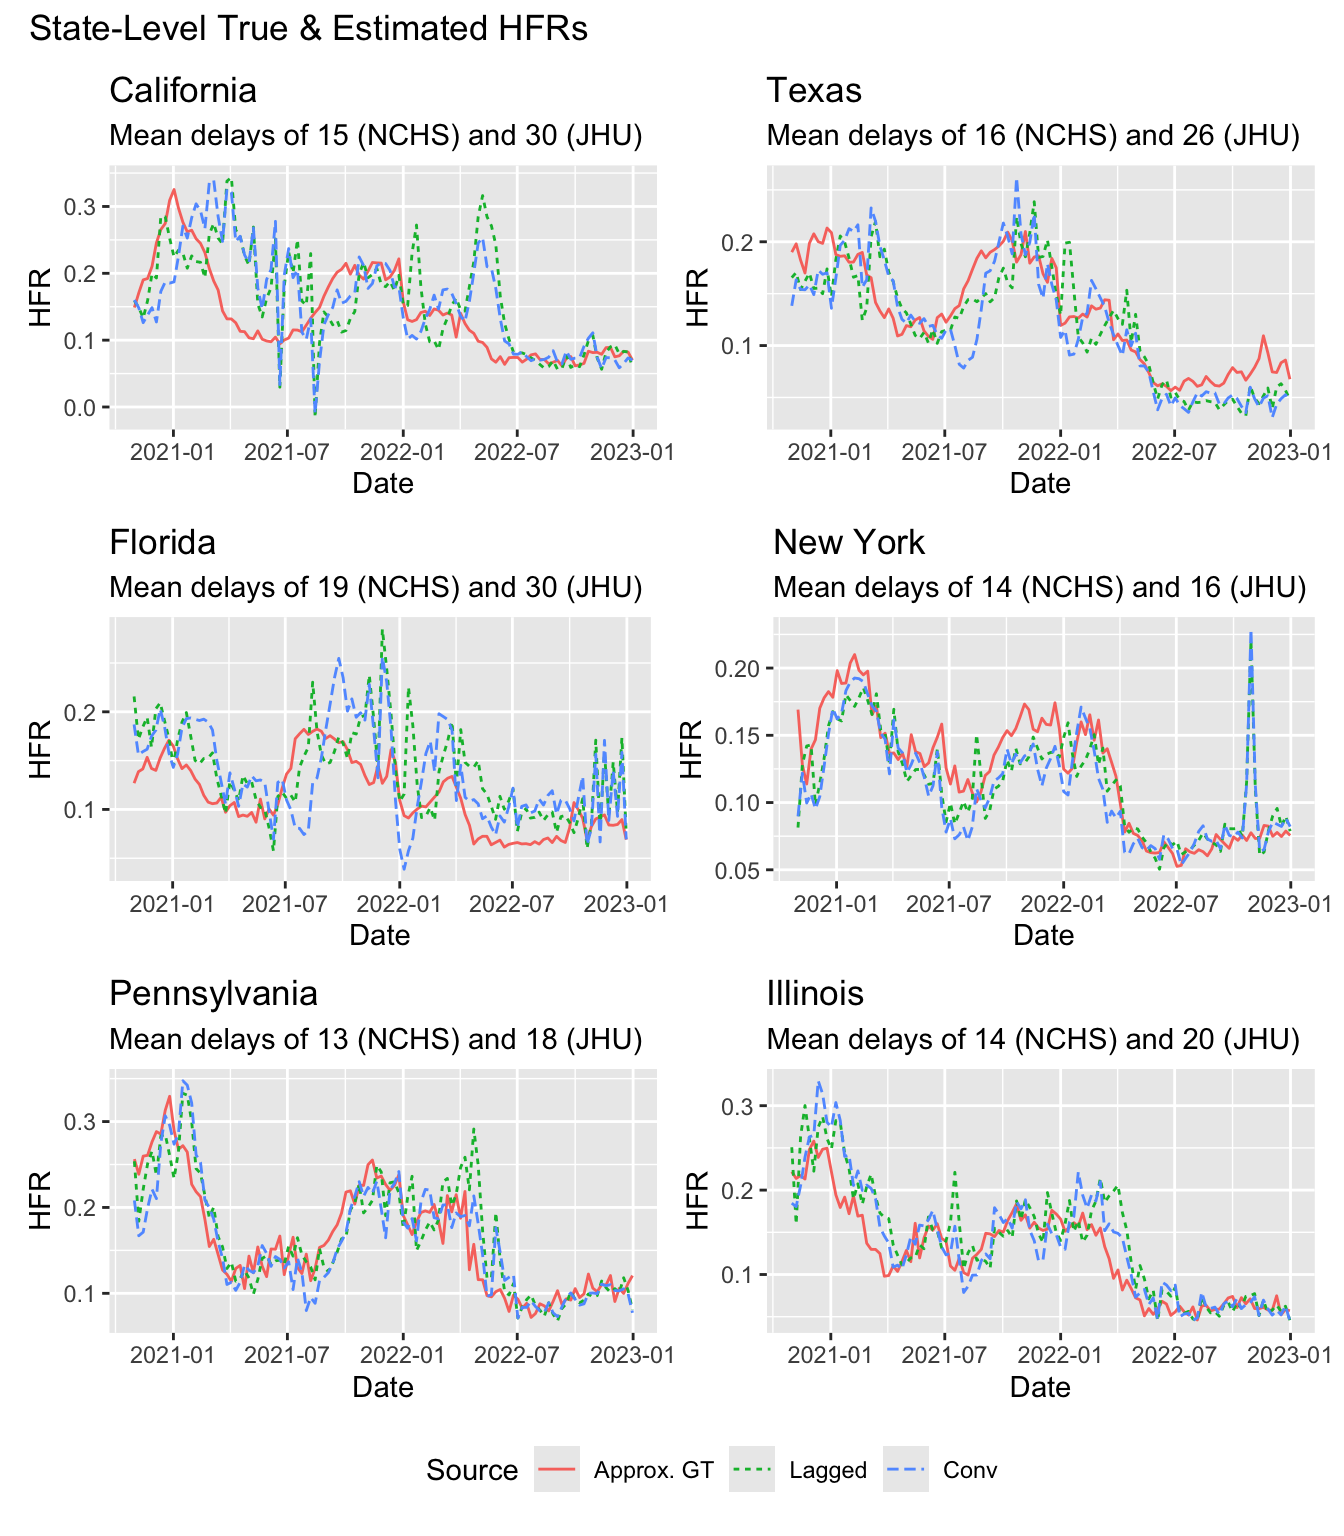
\includegraphics[width=0.8\linewidth]{Figs/state_level_hfrs.png}
     \caption{HFRs by individual states. Comparing retrospective estimates with NCHS against real-time estimates with JHU.}
     \label{fig:state-level}
 \end{figure}

Several states have similar biases as the US results (Fig. \ref{fig:basic_est_vs_gt}). Ratios in California, Texas, and Florida all are slow to detect the uptick in HFR during Delta; in California and Florida they also spike during Omicron. Note these states are the ones with the largest optimal lags, an estimate of the average time to death. As our simulated examples have shown, the shape of the delay distribution is a key factor behind the degree of bias. In contrast, New York, Pensylvania, and Illinois have mean delays of at most 20; while their HFRs are still biased, they are relatively close to the NCHS curve. This suggests that fatality ratios are generally less trustworthy in states that take longer to report deaths.


\end{document}
